\begin{figure*}
    \centering
	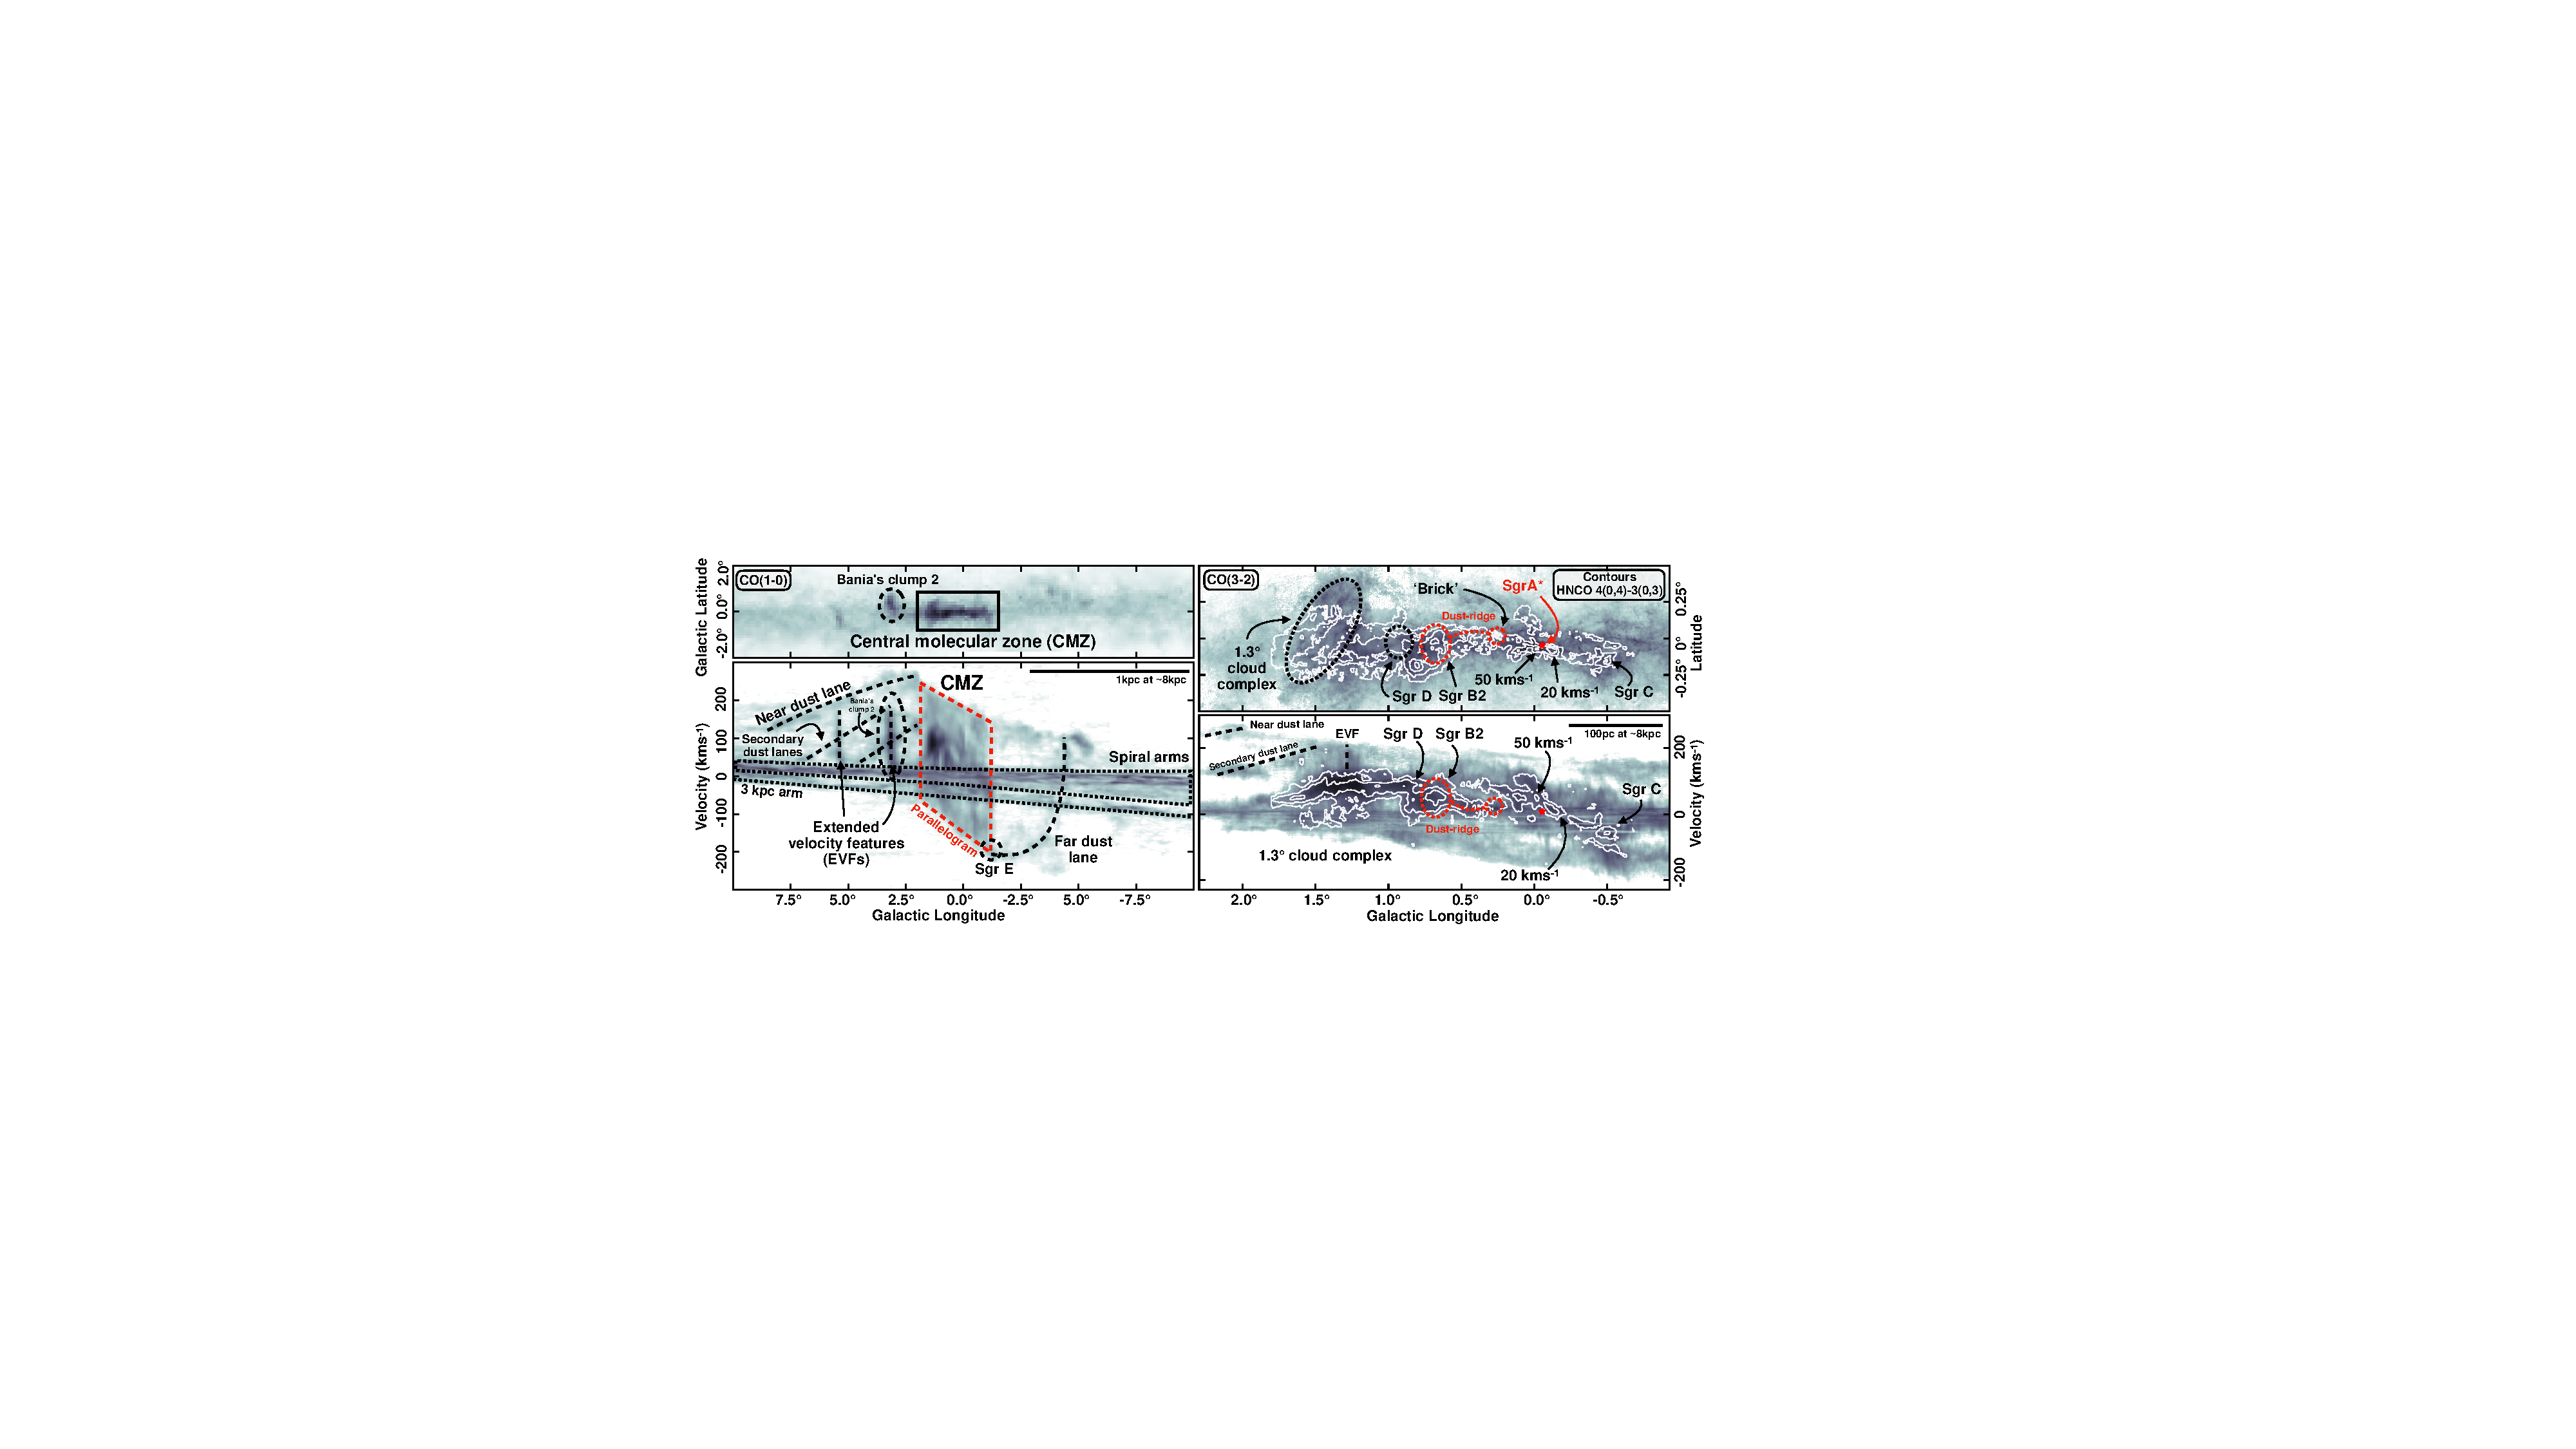
\includegraphics[trim=0 0cm 0 0cm, clip, width=0.9\textwidth]{./figs/lbv_compressed_v3.pdf}
    \caption{Atlas of the position-position-velocity ($\{l,b,v\}$ space) structure within the centre of the Milky Way. 
    The left panels show the integrated intensity of the $^{12}$CO $J=1-0$ line across the central few degrees ($\sim\,$ few kpc) of the Galaxy \citep{Dame2001}.
    The right panels show the integrated intensity of the $^{12}$CO $J=3-2$ line across the inner degree ($\sim\,$~300\,pc) taken as part of the CHIMPS2 survey \citep{Eden2020}.
    Overlaid as white contours is the HNCO\,$4(0,4)\mhyphen3(0,3)$ emission, a tracer of denser gas, taken as part of the Mopra CMZ survey \citep{Jones2012}.
    Labelled on both sets of panels are the prominent features discussed throughout this review (see in particular \S\ref{sec:IG} for the taxonomy of the inner Galaxy, and \S\ref{sec:massreservoir} for a detailed discussion of structures in the CMZ). The horizontal stripes in the CO emission shown in bottom-right panel are absorption from foreground spiral arms.}
    \label{fig:lbv_main}
\end{figure*}